\section{Results}\label{Sec:Results}

\subsection{Sample Preparation}

Before pooling the adaptor-ligated and indexed sequencing libraries, the sucess of
library preparation is validated using the Agilent Bioanalyzer instrument. \ref{fig:f1}
and \ref{fig:f2} show representative electropherograms of a sample that has been
processed using both kits. The expected DNA products should be detected at 175-600 bp
for Haloplex CSC and 200-400 for TST15.

\begin{figure}[!htbp]
  \centering
  \subfloat[Agilent Haloplex CSC (High Sensitivity DNA Chip)]{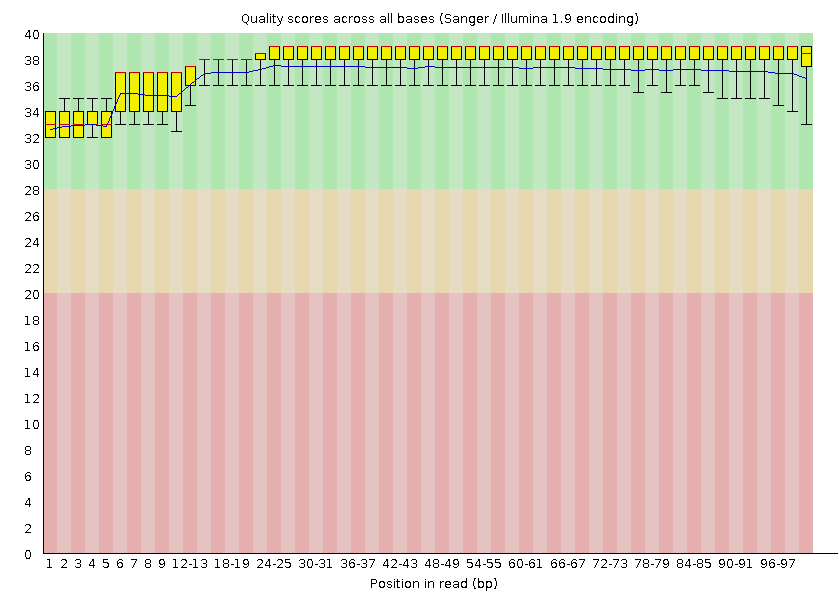
\includegraphics[width=0.45\textwidth]{fastq_halo_forward.png}\label{fig:f1}}
  \hfill
  \subfloat[Illumina TST15 (MixA) (DNA 1000 DNA Chip)]{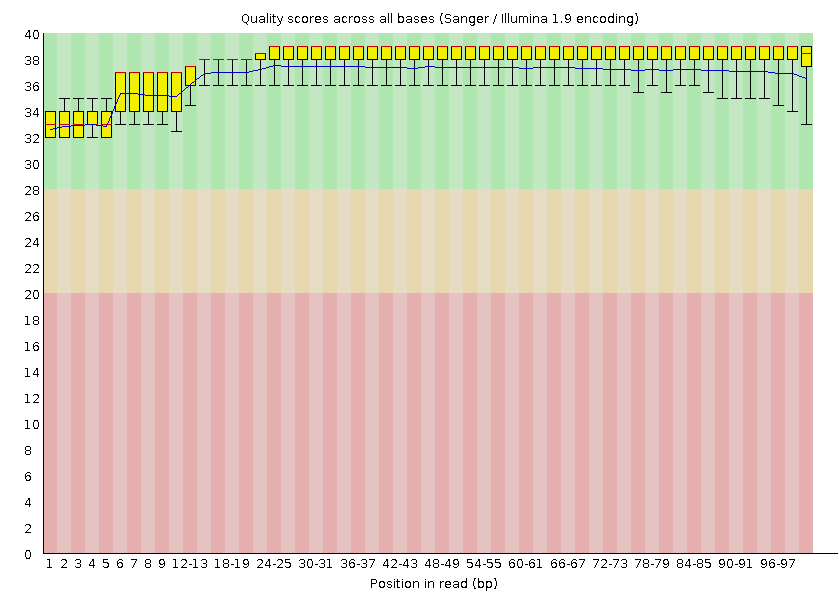
\includegraphics[width=0.45\textwidth]{fastq_halo_forward.png}\label{fig:f2}}
  \caption{Electropherograms of representative sequencing libraries prepared by Agilent Haloplex ClearSeq Cancer and Illumina TruSight Tumor 15. (*) represents the lower marker, (**) represents the upper marker}
\end{figure}

\begin{figure}[!htbp]
  \begin{center}
    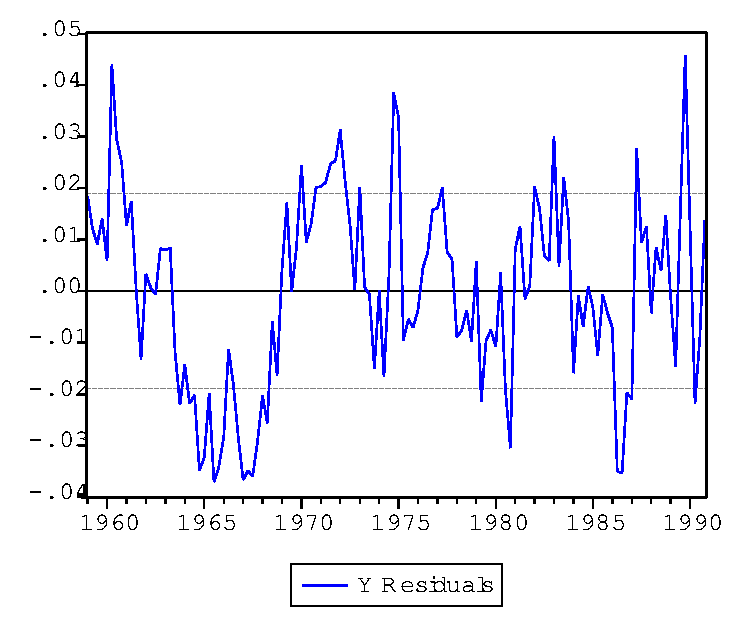
\includegraphics[scale=0.75,angle=0]{graph.pdf}
    \caption{Scatter plot of the corrected peak area (X axis) of the regions corresponding to the sequencing libraries defined in the blabla software and the dCt (Y axis). Agilent Haloplex ClearSeq Cancer data are represented as blue dots, Illumina TruSight Tumor 15 data are represented as red dots.}
    \label{Fig:bioanalyzer_scatter}
  \end{center}
\end{figure}

Using the blablabla software, the concentration, molarity and total peak area (TPA)
of the expected sequencing libraries were calculated.

Maybe: relationship between dCt and TPA?

Maybe: the enrichment of one or the other kit is more affected by bad quality samples

\subsection{NGS Data Quality}

Sequencing run parameters were calculated by the Illumina Sequencing Viewer software.
Table XXX shows the averaged run parameters of runs with Haloplex CSC and TST15
sample preparation.

\begin{table}[!htbp]
    \caption[ISV]{Comparison of Run Parameters (Averaged) of Sequencing Runs with Haloplex CSC \& TST15 Sample Preparation}
    \centering
    \begin{tabular}{ |p{4.5cm}|p{2cm}|p{2cm}|}
    \hline
    Parameter & Haloplex CSC & TST15 \\ \hline
    Yield total (Gb) & 3.7 & 7.37 \\
    \% \textgreater Q30 & 93.8 & 82.355 \\
    Cluster Density PF (k/mm2) & 1084 & 1180  \\
    Cluster Density PF (\%) & 85.95 & 79.95 \\
    \hline
    \label{sequencing_viewer}
  \end{tabular}
\end{table}

TST15 has a higher cluster density and therefore a higher total yield, but has
lower reads passing a phred-score threshold of Q30 than Haloplex. This is due to
the different chemistries used. TST15 uses v3 chemistry, while Haloplex uses v2.
v2 generally has lower cluster density and output, but therefore better quality.

\begin{figure}[!tbp]
  \centering
  \subfloat[Agilent Haloplex ClearSeq Cancer]{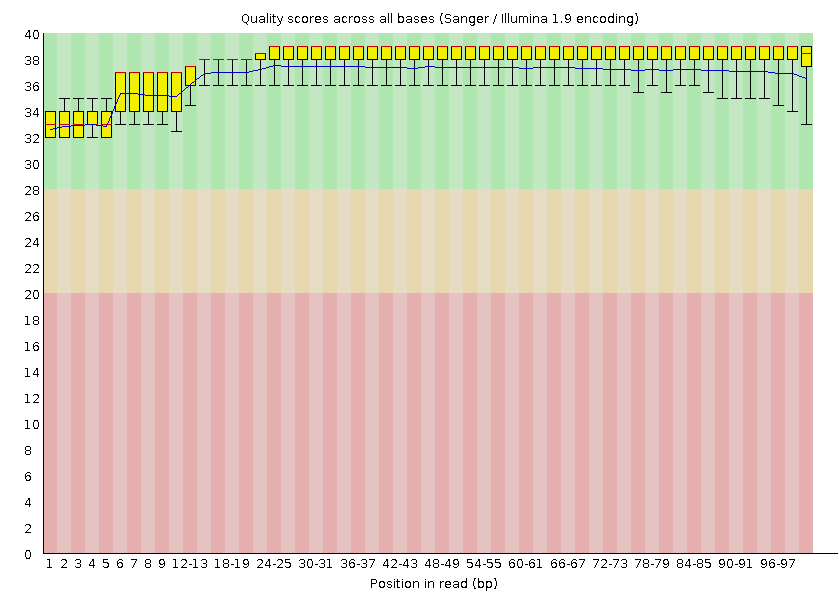
\includegraphics[width=0.5\textwidth]{fastq_halo_forward.png}\label{fig:amp_dist_hpx}}
  \hfill
  \subfloat[Illumina TruSight Tumor 15]{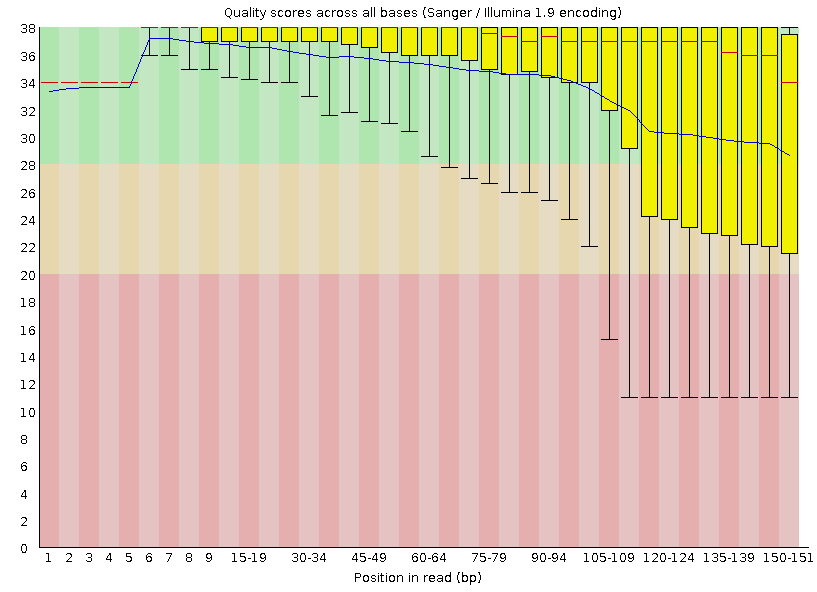
\includegraphics[width=0.5\textwidth]{fastq_tst15_forward.png}\label{fig:amp_dist_tst}}
  \caption{Comparison of coverage distributions per amplicon as reported by FastQC}
\end{figure}

Table XXX shows the boxplot representations of the read qualities per position
of two representative FASTQ files as reported by FastQC. Both workflows yield high
quality data, yet Haloplex CSC data have more narrow distributions and are of higher
quality. This is in direct relationship with the sequencing chemistry kit used.

\begin{table}
\begin{tabular}{p{3.5cm} p{1cm} p{1cm}}\\
\hline
Parameter & Halo CSC & Halo CSC & Halo CSC & TST15 & TST15 \\
          & SureCall duplicates removed & SureCall & Velona & BaseSpace & Velona \\
\hline
\% mapped & & & & 62.6 & \\
\% paired & & & & 58.7 & \\
\% singletons & & & & 3.8 & \\
\label{samtools_flagstat}
\end{tabular}
\end{table}

The Samtools Flagstat command was used to determine some basic BAM statistics of BAM
files of samples prepared with the respective library preparations and processed with
the mentioned bioinformatic pipelines. \ref{table:samtools_flagstat} shows the
averaged result of these statistics.

Considering the recommended pipelines, Haloplex
CSC data, analyzed with Agilent's SureCall software, has a higher percentage (91\%) of mapped
reads when compared to Illumina's BaseSpace TruSight Tumor 15 App (62.9\%). Data analysis
with the recommended SureCall design includes a steps where mates are fixed, but they
are not stitched together. Therefore no reads are considered as being paired. The TST15 app
in contrast includes a read stitching step and 58\% are considered as properly paired.
This means that of the 62.6\% of mapped reads, 4.2\% are not properly paired. 3.8\%
of reads processed with the TST15 online App are considered to be singletons, whereas
only 1.8\% of reads processed with the SureCall software are considered as singletons.

\subsection{Coverage Analysis}

Coverage Distribution TST15 vs Haloplex

Coverage Distribution per Patient (check if correlation IQR with dCt)

Coverage Distribution per Amplicon (check if some have always lower coverage, check if some failed)
\begin{figure}[!tbp]
  \centering
  \subfloat[Agilent Haloplex ClearSeq Cancer]{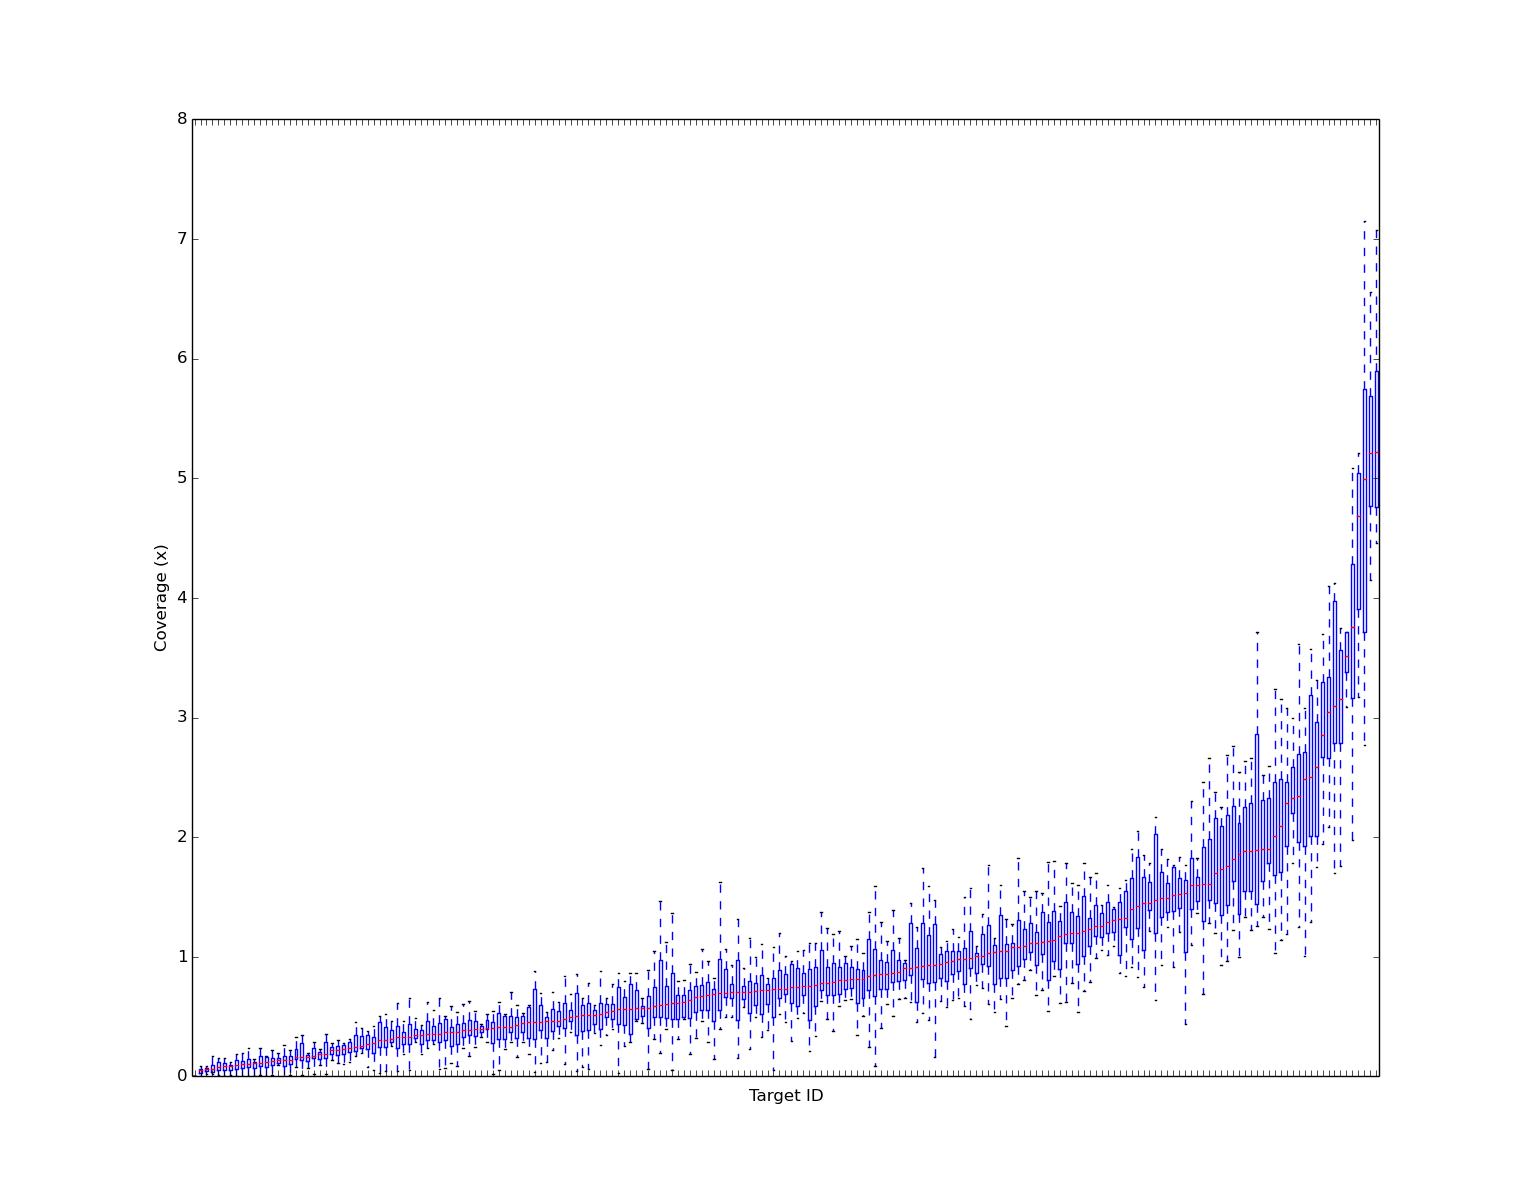
\includegraphics[width=0.5\textwidth]{distribution_amplicons_hap_csc.png}\label{fig:amp_dist_hpx}}
  \hfill
  \subfloat[Illumina TruSight Tumor 15]{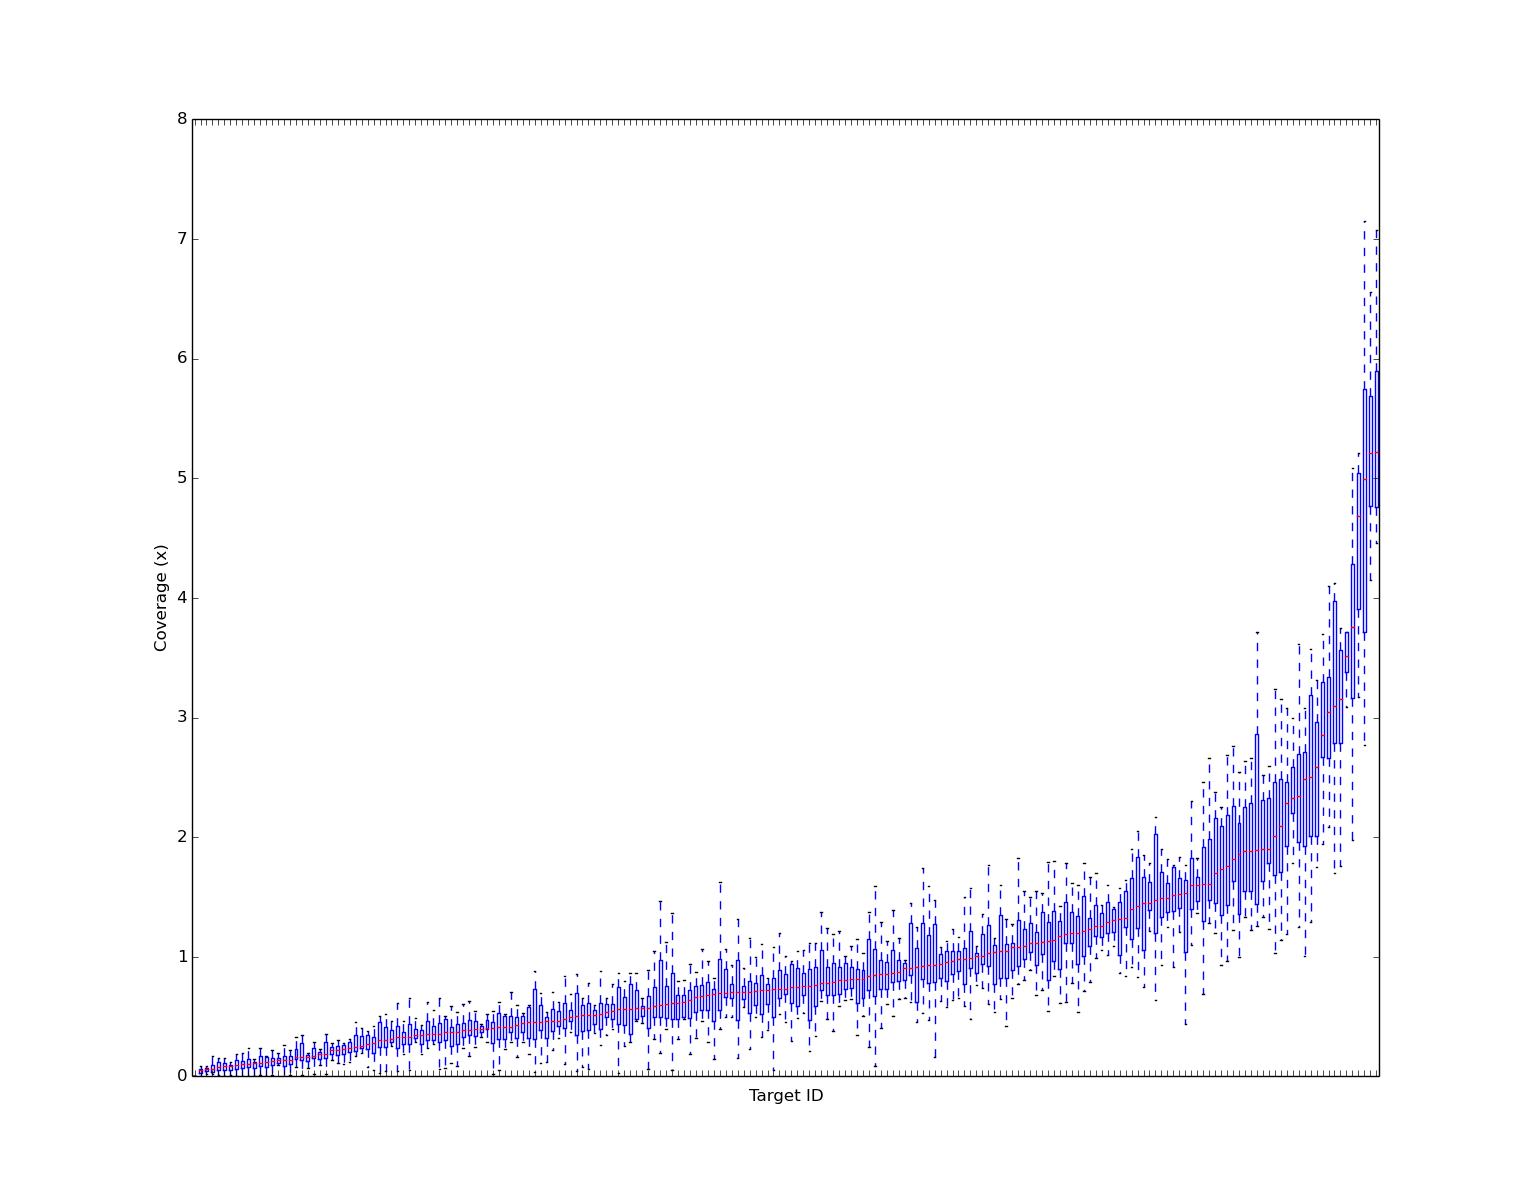
\includegraphics[width=0.5\textwidth]{distribution_amplicons_hap_csc.png}\label{fig:amp_dist_tst}}
  \caption{Comparison of Coverage Distributions per Amplicon}
\end{figure}

% Merge TST15 MixA & MixB together in one figure.
% Try to extract median values out of boxplots; new figure with these points
% -> some kind of trend line. The sooner it gets to a normalized coverage value of 1,
% the better.

% Looks like TST15 are better than Haloplex. But problem in TST: some EGFR & KRAS
% have low distributions.

% Do the same for EGFR; KRAS; NRAS; BRAF

Failed Amplicon Counter

\begin{minipage}{0.5\textwidth}
\captionof{table}{Failed Amplicons in Agilent Haloplex ClearSeq Cancer}
\begin{tabular}{p{3cm} p{1.5cm} p{1.5cm}}\\
\hline
Amplicon & Coverage Failed & No of Samples \\
\hline
ATM\_14 & 1 & all \\
Bla & 200 & 9 \\
Blabla & 500 & 5 \\
\label{failed_hpx}
\end{tabular}
\end{minipage}
\hfill
\begin{minipage}{0.5\textwidth}
\captionof{table}{Failed Amplicons in Illumina TruSight Tumor 15}
\begin{tabular}{p{3cm} p{1.5cm} p{1.5cm}}\\
\hline
Amplicon & 1x & 50x & 250x & 500x & 1000x \\
\hline
1METxxxE16TF031SR031 & 0 & 11 & 0 & 1 & 3 \\
17qxxxxExxTF018SR018 & 0 & 1 & 1 & 4 & 4 \\
1KRASxxE04TF002SR002 & 0 & 1 & 1 & 3 & 6 \\
1TP53xxE02TF034SR034 & 0 & 0 & 3 & 5 & 9 \\
1EGFRxxE19TF032SR032 & 0 & 0 & 1 & 5 & 5 \\
1EGFRxxE21TF035SR035 & 0 & 0 & 1 & 2 & 2 \\
\label{failed_tst}
\end{tabular}
\end{minipage}

Table XXX and table XXX show how often a given amplicon failed a given coverage
threshold. The number of failed amplicons is low for Haloplex CSC as wel las for TST15.
Most amplicons were amplified efficiently in most samples. Most counts in this
table originate from sample G, which, as already mentioned, had a bad dCt. Even
though this table shows that there are only a few amplicons failing the respective
coverage thresholds, the following issues were observed:
\begin{itemize}
\item Amplicon ATM\_14 was never amplified in Haloplex CSC data.
\item Amplicon blabla problem mat kras an egfr failed

\end{itemize}

ATM\_14 is never amplified in Haloplex CSC data.

Fragmentation <-> Coverage?
% Scatter plot: dCt vs normalized coverage (median / IQR ???)

(GATK CallableLoci)
(GATK CountLoci???)
(GATK FindCoveredIntervals)

On-off target; Enrichment Efficiency TST15 vs Haloplex

Coverage across genome, check where there is coverage

Strandedness?

GATK DepthOfCoverage???

\subsection{Variant Calling Algorithm Comparison}

\subsubsection{Detection of Known Single Nucleotide Variants and Deletions}

Table XXX shows known variants in the analyzed samples and the variant frequency
reported by the recommended pipelines. There is a high concordance between  the
results of both kits and previously known variants.

TST15 could not detect EGFR del19 in patient F due to low coverage. The
corresponding region was inspected in IGV and the deletion was present.  The
amplicon was not amplified  efficiently and has only a coverage of 167x. The
TST15 BaseSpace App however  applies a coverage threshold at 500x. Variants with
a lower depth are not reported. The same sample was sequenced twice and the
deletion was never detected. This is probably due to the fragmentation induced
by the FFPE fixation.

Haloplex CSC did not find KRAS p.Gly12Val in patient G, also due to low coverage
for this amplicon. The corresponding region was inspected in IGV: the region has
a coverage of only 180x. Only one read showed the expected C>A variant.  Sample
G is also the sample with the worst dCt (2.85). The  hig fragmentation in this
sample is probably responsible for the bad amplification. The same sample will
be re-sequenced in a later run to check  is the problem is related to the
fragmentation of the sample or if library preparation was bad.

\begin{table}
\begin{tabular}{p{3.5cm} p{1cm} p{1cm}}\\
\hline
Sample_ID & Context & Tissue & Known variant & Halo CSC Freq (\%) & TST15 Freq (\%) \\
\hline
A & NSCLC & FFPE & EGFR L858R & 24.7 & 21.4 \\
B & NSCLC & FFPE & EGFR L858R & 24.3 & 13.2 \\
C & NSCLC & FFPE & EGFR L858R & 32.7 & 29.8\\
D & Melanoma & FFPE & BRAF V600E & 44.4 & 47.6 \\
E & mCRC & FFPE & BRAF V600E & 18.4 & 21.4 \\
F & NSCLC & FFPE & EGFR del19 & not_found & 50 \\
G & mCRC & FFPE & KRAS CD 12_13 & p.Gly12Val (3.4) & not_found \\
H & mCRC & FFPE & KRAS CD 12_13  & p.Gly12Asp (37.4) & G12D (31.4)\\
I & mCRC & FFPE & KRAS CD 12_13  & p.Gly13Asp (9.7 )& G13D (8.7) \\
J & mCRC & FFPE & NRAS p.Gly12Asp & 25.9 & 27.2 \\
K & Melanoma & FFPE & BRAF V600E & 66.2 & 59.5 \\
L & mCRC & FFPE & NRAS p.Gly13Val & 6.6 & 5 \\
M & mCRC & FFPE & KRAS and NRAS WT & WT & WT \\
N & mCRC & FFPE & KRAS and NRAS WT & WT & WT \\
O & Melanoma & FFPE &BRAF V600E & 37.4 & \\
\label{known_variants}
\end{tabular}
\end{table}

Additional previously unknown variants were found (TODO: put a table into the appendix)

\subsubsection{Sensitivity Analysis}
BRAF Mut and WT samples from Horizon were analyzed. The BRAF Mut sample was
sequenced purely, as well as in a 1/3 and 2/3 dilution with the BRAF WT sample.

\begin{table}
\begin{tabular}{p{3.5cm} p{1cm} p{1cm}}\\
\hline
Gene & Variant & Expected Var Freq 100\% &  Var Freq 100\% Halo CSC &  Var Freq 100\% TST 15 & Expected Var Freq 66\% &  Var Freq 66\% Halo CSC & Expected Var Freq 66\% TST15 & Expected Var Freq 33\% & Var Freq 33\% Halo CSC & Var Freq 33\% TST15 \\
\hline
BRAF & V600E & 10.5 & & 12.5 & 7 & & 8.3 & 3.5 & & 4.4 \\
cKIT & D816V & 10 & & -- & 6.67 & & -- & 3.33 & & -- \\
EGFR & delE756-A751 & 2 & & -- & 1.33 & & -- & 0.67 & & -- \\
EGFR & L858R & 3 & & 3.6 & 2 & & -- & 1 & & -- \\
EGFR & T790M & 1 & & -- & 0.67 & & -- & 0.33 & & -- \\
EGFR & G719S & 24.5 & & 24.2 & 16.33 & & 18.9 & 8.17 & & 11.5 \\
KRAS & G13D & 15 & & 15.2 & 26.67 & & 27.7 & 38.33 & & 38.5 \\
KRAS & G12D & 6 & & 7.3 & 4 & & 3.3 & 2 & & -- \\
NRAS & Q61K & 12.5 & & 11.6 & 8.33 & & 8.3 & 4.17 & & 3.6 \\
PIK3CA & H1047R & 17.5 & & 16.1 & 26.67 & & 29.7 & 38.33 & & 37.9 \\
PIK3CA & E545K & 9 & & 7.6 & 6 & & 4.8 & 3 & & -- \\
\label{horizon_analysis}
\end{tabular}
\end{table}

The observed variant frequencies as detected by the TST15 BaseSpace App are
in line with the expected variant frequencies.

TODO: do the same with Haloplex CSC

TODO: call variants with MuTect 1.1.7, VarScan 2, GATK HaplotypeCaller, SomVarIUS?, Freebayes?, Vardict???????
TODO: compare results

Among the variants detected by MuTect, 40--50 \% are C>T variants. This has been reported in several studies.
TODO: do this for all samples, check if this is really statistically significant or only happened in a few samples

Tools that may be of use somehow: GATK SelectVariants; GATK VariantFiltration; GATK VariantEval; GATK ValidateVariants
